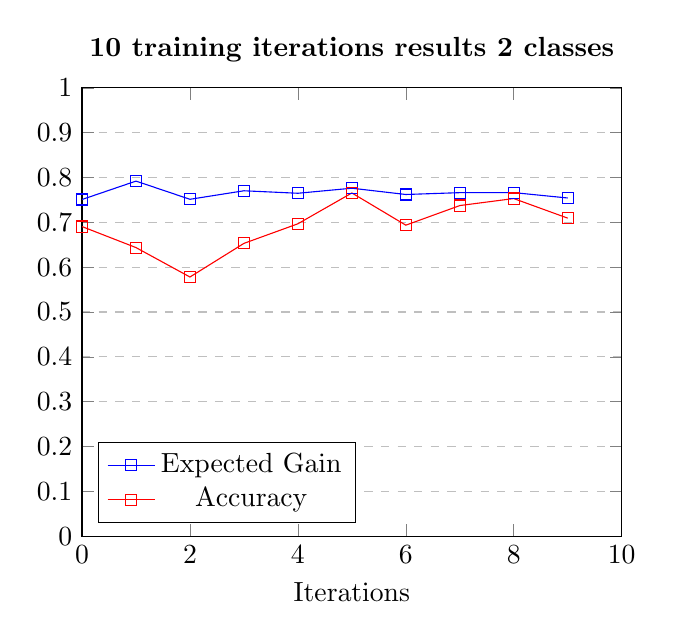
\begin{tikzpicture}
  \begin{axis}[
      title=\textbf{10 training iterations results 2 classes},
      xlabel={Iterations},
      xmin=0, xmax=10,
      ymin=0.0, ymax=1,
      xtick={0,2,4,6,8,10},
      ytick={0.0,0.1,0.2,0.3,0.4,0.5,0.6,0.7,0.8,0.9,1.0},
      legend pos=south west,
      ymajorgrids=true,
      grid style=dashed,
  ]

  \addplot[color=blue, mark=square]
    coordinates {
      (0, 0.7510161862543873)
      (1, 0.7920788037709293)
      (2, 0.7514642101011255)
      (3, 0.7704808259436531)
      (4, 0.7649375191939426)
      (5, 0.776186768335381)
      (6, 0.7621880262547054)
      (7, 0.7662678293114988)
      (8, 0.766369437713792)
      (9, 0.7543597171481017)
    };
    \addlegendentry{Expected Gain}
  
  \addplot[color=red, mark=square]
    coordinates {
      (0, 0.690625)
      (1, 0.64375)
      (2, 0.578125)
      (3, 0.653125)
      (4, 0.696875)
      (5, 0.765625)
      (6, 0.69375)
      (7, 0.7375)
      (8, 0.753125)
      (9, 0.709375)
    };
    \addlegendentry{Accuracy}
      
  \end{axis}
\end{tikzpicture}